% Appendix A

\chapter{Cálculos auxiliares} % Main appendix title

\label{AppendixA} % For referencing this appendix elsewhere, use \ref{AppendixA}

\lhead{Appendix A. \emph{Cálculos auxiliares}} % This is for the header on each page - perhaps a shortened title

\section{Cantidad de acoplamientos mutuos}

A continuación se muestran los cálculos realizados para poder determinar la cantidad de acoplamientos mutuos entre módulos
radiantes.

La cantidad de acoplamientos mutuos no depende de la geometría de la disposición de los elementos radiantes, simplemente de 
la cantidad de los mismos. Otra característica es, que el acoplamiento es la atenuación y defasaje que modifica la señal 
que va de una antena hacia otra, independientemente de si la primera transmite y la segunda recibe o viceversa 
($C_{12} = C_{21}$).

Asumiendo que se poseen $n$ módulos radiantes en línea, numeradors de 1 a $n$, como se muestra en la figura \ref{fig:RmsInARow},
se procederá a calcular todos los pares que hayan. 

\begin{figure}[H]
 \centering
 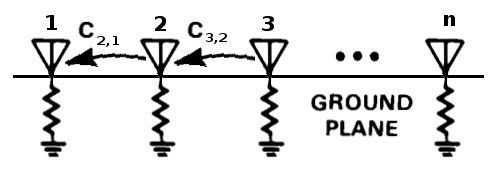
\includegraphics[width=6cm]{gfx/mutualCoupling.png}
 \caption{Acoplamientos mutuos entre módulos radiantes}
 \label{fig:RmsInARow}
\end{figure}

Pares que están a distancia de 1, o pares contiguos, son: $C_{12}$, $C_{23}$, $C_{34}$, ..., $C_{n_{-1}n}$. Por lo tanto se puede deducir
que son $n - 1$ acoplamientos.

Pares que están a distancia de 2: $C_{13}$, $C_{24}$, $C_{35}$, ..., $C_{n_{-2}n}$. Por lo tanto se puede deducir que son $n - 2$ acoplamientos.

Pares que están a distancia de 3: $C_{14}$, $C_{25}$, $C_{36}$, ..., $C_{n_{-3}n}$. Por lo tanto se puede deducir que son $n - 3$ acoplamientos.

Pares que están a distancia de $n - 1$: $C_{1n}$. Por lo tanto se puede deducir que es solo 1 acoplamiento. 

Generalizando, la cantidad de acoplamientos resulta ser 

\begin{equation}\label{eq:amountMutCoupling}
	\sum_{i = 1}^{n-1} i = \dfrac{n(n-1)}{2}
\end{equation}
